\documentclass{article}
\usepackage[utf8]{inputenc} % allow utf-8 input
\usepackage[main=english,russian]{babel}	
\usepackage{arxiv}

\usepackage[T1]{fontenc}    % use 8-bit T1 fonts
\usepackage{hyperref}       % hyperlinks
\usepackage{url}            % simple URL typesetting
\usepackage{booktabs}       % professional-quality tables
\usepackage{amsfonts}       % blackboard math symbols
\usepackage{nicefrac}       % compact symbols for 1/2, etc.
\usepackage{microtype}      % microtypography
\usepackage{lipsum}         % Can be removed after putting your text content
\usepackage{graphicx}
\usepackage{natbib}
\usepackage{doi}
\usepackage{amsmath}
\usepackage{algorithm}
\usepackage{algpseudocode}
\usepackage{amsthm}
\usepackage{amssymb}
\newtheorem{theorem}{Theorem}

\title{On the problem of repeated supervised learning}

%\date{September 9, 1985}	% Here you can change the date presented in the paper title
%\date{} 					% Or removing it

\author{
    Andrey S. Veprikov\\
	Department of Intelligent Systems\\
	MIPT\\
	Dolgoprudny, Russia \\
	\texttt{veprikov.as@phystech.edu} 
    \And
    Anton S. Khritankov\\
    HSE University\\
    Moscow, Russia\\
    \texttt{akhritankov@hse.ru}\\
    \And
    Alexander P. Afanasyev \\
    IITP\\
    Moscow, Russia}

\date{}

% Uncomment to override  the `A preprint' in the header
%\renewcommand{\headeright}{Technical Report}
%\renewcommand{\undertitle}{Technical Report}
\renewcommand{\shorttitle}{On the problem of repeated supervised learning}

%%% Add PDF metadata to help others organize their library
%%% Once the PDF is generated, you can check the metadata with
%%% $ pdfinfo template.pdf

\begin{document}
\maketitle

\begin{abstract}

    In this research paper, we delve into the intricacies of continuous learning artificial intelligence systems as they interact with and influence their environment. We develop a mathematical model to examine the process of repeated and multiple learning, prediction, and dataset updating. Our investigation of this process is based on the principles of functional analysis and probability theory, which is a novel approach to this problem. We aim to conduct several synthetic experiments based on our findings, hoping to contribute to a better understanding of the behavior of continuous learning AI systems.

\end{abstract}


% keywords can be removed
\keywords{Machine learning \and Continuous machine learning \and Repeated learning}

\section{Introduction} \label{Introduction}

    In this paper we consider the problem of repeated supervised learning \begin{otherlanguage}{russian}(многократное машинное обучение)\end{otherlanguage}, in which the training sample is not fixed, but is updated depending on the predictions of the trained model on the test sample \cite{ma2020machine, khritankov2021existence, jiang2019degenerate}. In many applications, the use of multiple learning techniques can actually lead to suboptimal results. Our main goal was to present a mathematical theory that explains why combining multiple learning algorithms can sometimes hinder their effectiveness. Repeated supervised learning appears in many machine learning applications, for example in recommendation systems \cite{khritankov2021existence, sinha2016deconvolving}, healthcare \cite{adam2020hidden} and predictive policing \cite{ensign2018runaway}. 

    The object of our research will be the set $\mathbf{R}$ of distribution density functions

    \begin{equation}
        \label{R}
        \mathbf{R} := \left\{f : \mathbb{R}^n \rightarrow \mathbb{R}_+ ~\text{and}~ \int\limits_{\mathbb{R}^n}f(x)dx = 1\right\}
    \end{equation}

    and a mapping $\text{D}$, a feedback loop mapping, that includes training a model, forming predictions on a test sample and mixing predictions into a training sample, as a result of which the distribution of features changes.

    In this paper we propose a mathematical model of the process of repeated learning that is new to the literature. We find sufficient conditions for the operator $\text{D}$ to translate $\mathbf{R}$ into $\mathbf{R}$. We find conditions for our data density functions to tend in a weak sense to a delta function under the operator $\text{D}$. We also find sufficient conditions for the operator $\text{D}$ to be non-contraction in the norm $\|\cdot \|_q$. The importance of these properties is explained in detail in Section \ref{Main_results}.
    
    Structure of this paper are as follows. In Section \ref{Related_work} we compare our article with the works of other authors and show its novelty to the literature. In Section \ref{Problem_statement} we build a mathematical model for the process of multiple learning, prediction and updating of the sample and outline the main questions, the answers to which we explore in Section \ref{Main_results}. In Section \ref{Main_results} we provide our main contributions for the mapping $\text{D}$. In Section \ref{Experiments}, based on the results from Section \ref{Main_results}, we conduct some synthetic experiments.

\section{Related work} \label{Related_work}    

    The problem we study is somewhat related to the feedback loops \cite{khritankov2021hidden, khritankov2021existence} -- an observable change in the distribution of input data that occurs over time, because of user interaction with the system. According to Conjecture 1 from \cite{khritankov2021hidden} the positive feedback loop in a system $\text{D} : R \rightarrow R$ exists if $\text{D}$ is a contraction mapping, but this conjecture was not proved.

    Also our problem is connected with dynamical systems, which are studied in \cite{katok1995introduction, nemytskii2015qualitative}, but all these works consider continuous time, and in our work it should be discrete.

    Some authors analyzed Markov processes from the point of view of dynamical systems \cite{tarlowski2017global, vershik2005does}. But in Markov chain the future of the process does not depend on the past. Other authors \cite{varvenne2019rate, pap1996fixed} studied stochastic dynamics systems in general.

    An important contribution of this paper is that  we built a mathematical model for continuous machine learning problem, which is novel to the literature.

\section{Problem statement} \label{Problem_statement}

    We consider $\mathbf{R}$ \eqref{R} -- the set of distribution density functions and a mapping $\text{D}$ representing an algorithm for training a model, forming predictions on a test sample and mixing predictions into a training sample, as a result of which the distribution of features changes.

    Let's consider an autonomous (time-independent explicitly) discrete dynamical system. There is a dedicated variable - the step number, which increases, at step $t$ and $t+1$ of which the ratio is fulfilled

    \begin{equation*}
        f_{t+1}(x) = \text{D}(f_t)(x), \quad \text{for}~ \forall x \in \mathbb{R}^n,
    \end{equation*}

    where $\text{D}$ becomes an evolution operator on the space of the specified functions $f$ and the initial function $f_0(x)$ is known. Generally speaking, $\text{D}$ can be an arbitrary mapping, not necessarily smooth or continuous.


    In the next section, we provide several conditions on the operator $\text{D}$, in order for it to translate $\mathbf{R}$ into $\mathbf{R}$. It is important, because we consider $\text{D}$ as operator of changing distribution of our dataset, so it has to transform $\mathbf{R}$ into $\mathbf{R}$.

    We also look at the conditions under which the data density functions will tend to a delta function in the weak sense, i.e. $\text{D}^t(f_0)(x) \underset{t \to +\infty}{\longrightarrow} \delta(x)$. 
    This is an important property, because we it can be used to understand when repeated machine learning improves our metrics. Why this is so will be discussed in detail in Section \ref{Main_results}.

    Another contribution of our paper is a condition, under that operator $\text{D}$ wouldn't be a contraction mapping in any norm $\|\cdot\|_q$, i.e. there always would be function $f \in \mathbf{R}$ such that $\|\text{D}(f)\|_q \geq \|f\|_q$. This is also important property, because if $\text{D}$ is a contraction mapping, then it converge any start density distribution $f_0$ to function that is equal to zero in almost every point $x \in \mathbb{R}^n$, i.e. continuous algorithm transform our data to uniform noise.


\section{Main results} \label{Main_results}

    \textbf{Notation:} In this paper we will use the common notations: the $L_1(\mathbb{R}^n)$-norm of function $f$:

    \begin{equation*}
        \|f\|_1 := \int\limits_{\mathbb{R}^n} |f(x)| dx \quad \text{ and } \quad L_1(\mathbb{R}^n) := \left\{f : \mathbb{R}^n \to \mathbb{R} ~|~ \|f\|_1 < + \infty\right\}
    \end{equation*}

    The $L_{\infty}(\mathbb{R}^n)$-norm of function $f$:

    \begin{equation*}
        \|f\|_{\infty} := \underset{x \in \mathbb{R}^n}{\text{esssup}}\{f(x)\} := \inf\{C \geq 0 ~|~ |f(x)| \leq C \text{ for almost every } x \in \mathbb{R}^n\} \quad \text{ and } \quad L_{\infty}(\mathbb{R}^n) := \left\{f : \mathbb{R}^n \to \mathbb{R} ~|~ \|f\|_{\infty} < + \infty\right\}
    \end{equation*}

    \begin{theorem}[Fact] \label{based}
        If $f: \mathbb{R}^n \to \mathbb{R}$ such that $f(x) \geq 0$ for almost every $x \in \mathbb{R}^n$ and $\|f\|_1 = \int\limits_{\mathbb{R}^n} f(x) dx = 1$, then there exists a random vector $\mathbf{\xi}$, for which $f$ will be a density distribution function.
    \end{theorem}

    Exactly on the basis of Theorem \ref{based} we define $\mathbf{R}$ \eqref{R} in this way.

    \begin{theorem}[Assumptions for $\text{D}: \mathbf{R} \to \mathbf{R}$] \label{R_to_R}
        If $\|\text{D}\|_1 = 1, \forall f \in \mathbf{R} \hookrightarrow \text{D}(f)(x) \geq 0$ for almost every $x \in \mathbb{R}^n$, and exists $\text{D}^{-1}$ such that $\|\text{D}^{-1}\|_1 \leq 1$, then $\text{D} : \mathbf{R} \to \mathbf{R}$.
    \end{theorem}
    \begin{proof}
        To begin with, let us note that if $\text{D}: \mathbf{R} \to \mathbf{R}$, then $\|\text{D}\|_1 = 1$, because by definition of operator norm:

        \begin{equation*}
            \|\text{D}\|_1 \overset{def}{=} \underset{\|f\|_1 = 1}{\sup}\left\{\|\text{D}(f)\|_1\right\}
        \end{equation*}

        And if $f$ such that $\|f\|_1 = 1$ then $|f| \in \mathbf{R}$ and, because $\text{D}: \mathbf{R} \to \mathbf{R}$, $\|\text{D}(|f|)\|_1 = 1$. But $\|\text{D}\|_1 = 1$ is only a necessary but not a sufficient condition.

        If $\|\text{D}\|_1 = 1$, then $\forall f \in \mathbf{R} \hookrightarrow \text{D}(f) \leq 1$. If $\exists f_0 \in \mathbf{R}$ such that $\|\text{D}(f_0)\|_1 < 1$, then we get a contradiction because

        \begin{equation*}
            \|D^{-1}\|_1 \overset{def}{=} \underset{\|f\|_1 \neq 0}{\sup}\left\{\dfrac{\|\text{D}^{-1}(f)\|_1}{\|f\|_1}\right\} 
            \geq \left[f_1 = \text{D}(f_0)\right] \geq
            \dfrac{\|\text{D}^{-1}(f_1)\|_1}{\|f_1\|_1} = 
            \dfrac{\|\text{D}^{-1}(\text{D}(f_0))\|_1}{\|\text{D}(f_0)\|_1} = 
            \dfrac{\|f_0\|_1}{\|\text{D}(f_0)\|_1} = \dfrac{1}{\|\text{D}(f_0)\|_1} > 1
        \end{equation*}

        But we assume that $\|\text{D}^{-1}\|_1 \leq 1$. So $\forall f \in \mathbf{R} \hookrightarrow \|\text{D}(f)\|_1 = 1$.

        But according to Theorem \ref{R_to_R} to $\text{D} : \mathbf{R} \to \mathbf{R}$ we also need second assumption: $\forall f \in \mathbf{R} \hookrightarrow \text{D}(f)(x) \geq 0$ for almost every $x \in \mathbb{R}^n$.
        
    \end{proof}

    \textbf{Discussion of Theorem \ref{R_to_R}}

    In experiments it often difficult to calculate $\text{D}^{-1}$ and especially it's norm, so we make a different assumptions. We consider $\text{D}$ as algorithm for training a model, forming predictions on a test sample and mixing predictions into a training sample. Distribution of our data is approximating by empirical distribution function \cite{dvoretzky1956asymptotic} as follows (for $n=1$):

    \begin{equation}\label{F_approx}
        \hat{F}_N(x) := \dfrac{\text{number of elements in sample} \leq x}{N} = \dfrac{1}{N}\sum\limits_{i=1}^N \textbf{1}_{X_i \leq x},
    \end{equation}

    where $X_i$ are elements of sample. We assume that $(X_1, X_2, X_3, ... , X_N)$ are independent, identically distributed real random variables with the common cumulative distribution function $F(x)$. If this assumption is fulfilled, then the DKW inequality is satisfied:

    \begin{equation}\label{DKW}
        \mathbb{P}\left\{\underset{x \in \mathbb{R}}{\sup}\left|\hat{F}_N(x) - F(x)\right| > \varepsilon \right\} \leq C e^{-2N\varepsilon^2} \quad 
        \forall \varepsilon > 0
    \end{equation}

    And we can build interval that contains the true CDF of our data $F(x)$, with probability $1 - \alpha$ as

    \begin{equation}\label{inter}
        \hat{F}_N(x) - \varepsilon \leq F(x) \leq \hat{F}_N(x) + \varepsilon, ~~ \text{ where } ~~ \varepsilon = \sqrt{\dfrac{\ln(2/\alpha)}{2N}}
    \end{equation}

    In this case operator $\text{D}$ transoms our data, i.e. translates one empirical distribution function to another. So $\text{D} : \mathbf{R} \to \mathbf{R}$ by constructing our experiment.

    \begin{theorem}[Limit in a weak sense to $\delta$ function] \label{delta}
        If $f_t : \mathbb{R} \to \mathbb{R}$ such that $\forall t \in \mathbb{N} \hookrightarrow  \|f_t\|_1 = 1$, $f_t(x) \geq 0$ in almost every point $x \in \mathbb{R}$ and
        \begin{equation} \label{psi_and_g}
            \exists \psi : \mathbb{N} \to \mathbb{R} : \psi(t) \underset{t \to +\infty}{\longrightarrow} +\infty ~\text{ and }~
            \exists g \in L_1(\mathbb{R}) ~\text{ such that }~ \forall t \in \mathbb{N} ~\forall y \in \mathbb{R} \hookrightarrow f_t\left(\dfrac{y}{\psi(t)}\right) \leq \psi(t) \cdot |g(y)|
        \end{equation}

        Then $f_t(x) \underset{t \to \infty}{\longrightarrow} \delta(x)$ in a weak sense, i.e.

        \begin{equation}
            \underset{t \to +\infty}{\lim}\left(\int\limits_{-\infty}^{+\infty} f_t(x) \phi(x) dx\right) = \phi(0),
        \end{equation}

        where $\phi$ is continuous function with compact support
    \end{theorem}

    \begin{proof}
        Assume a notation $I_t = \int\limits_{-\infty}^{+\infty} f_t(x) \phi(x) dx$. Then it's fulfilled that

        \begin{equation*}
            I_t - \phi(0) = \int\limits_{-\infty}^{+\infty} f_t(x) \phi(x) dx - \phi(0) \cdot \int\limits_{-\infty}^{+\infty} f_t(x) dx = \int\limits_{-\infty}^{+\infty} f_t(x) \cdot [\phi(x) - \phi(0)] dx
        \end{equation*}

        The first equation is fulfilled because $\|f_t\| = 1$.
        
        Replacing the variable $y = \psi(t) \cdot x, dy = \psi(t) \cdot dx$ we get

        \begin{equation} \label{tmp2}
            I_t - \phi(0) = \dfrac{1}{\psi(t)} \cdot \int\limits_{-\infty}^{+\infty} f_t\left(\frac{y}{\psi(t)}\right) \cdot \left[\phi\left(\frac{y}{\psi(t)}\right) - \phi(0)\right] dy
        \end{equation}

        Split the integral \eqref{tmp2} into 3 parts:
        
        \begin{equation*}
            I_1 := \dfrac{1}{\psi(t)} \cdot \int\limits_{-\infty}^{-A} f_t\left(\frac{y}{\psi(t)}\right) \cdot \left[\phi\left(\frac{y}{\psi(t)}\right) - \phi(0)\right] dy
        \end{equation*}
        \begin{equation*}
            I_2 := \dfrac{1}{\psi(t)} \cdot \int\limits_{-A}^{A} f_t\left(\frac{y}{\psi(t)}\right) \cdot \left[\phi\left(\frac{y}{\psi(t)}\right) - \phi(0)\right] dy
        \end{equation*}
        \begin{equation*}
            I_3 := \dfrac{1}{\psi(t)} \cdot \int\limits_{A}^{+\infty} f_t\left(\frac{y}{\psi(t)}\right) \cdot \left[\phi\left(\frac{y}{\psi(t)}\right) - \phi(0)\right] dy
        \end{equation*}

        Consider the integrals $I_1$. $\phi$ is continuous function with compact support, so $\phi$ is bounded by some constant $M$, i.e. $\forall x \in \mathbb{R} \hookrightarrow |\phi(x)| \leq M$, so 

        \begin{equation*}
            \left|I_1\right| \leq \int\limits_{-\infty}^{-A} 2 M \cdot \dfrac{1}{\psi(t)} f_t\left(\frac{y}{\psi(t)}\right) dy \leq \left[\eqref{psi_and_g}\right]
            \leq \int\limits_{-\infty}^{-A} 2 M \cdot |g(y)| dy 
        \end{equation*}

        Since $g \in L_1(\mathbb{R})$, there exists some constant $A > 0$ such that $\left|I_1\right| \leq \varepsilon$. Similarly, it can be shown that $\left|I_3\right| \leq \varepsilon$.

        Consider the integral $I_2$. $\phi$ is continuous and $\psi \to +\infty$ \eqref{psi_and_g}, so $\exists~ T \in \mathbb{N}$ such that $\forall y \in [-A; A]$ $\forall t \geq T$ it is fulfilled that 

        \begin{equation*}
            \left|\frac{y}{\psi(t)} - 0\right| \leq \delta ~\text{ and so }~ \left|\phi\left(\frac{y}{\psi(t)}\right) - \phi(0)\right| \leq \varepsilon
        \end{equation*}

        So

        \begin{equation*}
            \left|I_2\right| \leq \varepsilon \cdot \int\limits_{-A}^{A} \dfrac{1}{\psi(t)} f_t\left(\frac{y}{\psi(t)}\right) dy = 
            \varepsilon \cdot \int\limits_{-A/\psi(t)}^{A/\psi(t)} f_t\left(x\right) dx \leq \varepsilon \cdot \int\limits_{-\infty}^{+\infty} f_t\left(x\right) dx = \varepsilon
        \end{equation*}

        Finally we get

        \begin{equation*}
            \forall \varepsilon > 0 ~~ \exists~ T \in \mathbb{N} : \forall t \geq T \hookrightarrow \left|I_t - \phi(0)\right| \leq 
            \left|I_1\right| + \left|I_2\right| + \left|I_3\right| \leq 3\varepsilon
        \end{equation*}

        So $f_t(x) \underset{t \to \infty}{\longrightarrow} \delta(x)$ in a weak sense.

    \end{proof}

    \textbf{Discussion of Theorem \ref{delta}}

    If in some step $t$ the model $H(x, \theta, t)$ starts to give good predictions on the training and test samples, then, in the probabilistic formulation, this means that the density function of the distribution of the object-sign vectors becomes similar to the delta function, as the components of the random vector $(\mathbf{x^i}, y_i) \subset (\mathbf{X}, \mathbf{y})$ become linearly dependent. Based on these considerations, we can compare each operator $\text{D}$ to an operator $\widetilde{\text{D}}$, where $\widetilde{\text{D}}$ transforms density distribution functions of random variables $\|\mathbf{y} - \mathbf{y_{\text{pred}}}\|$, where $\mathbf{y_{\text{pred}}} = H(\mathbf{X}, \theta, t)$. Then we can apply Theorem \ref{delta} to understand, when $\widetilde{\text{D}}(f_0)(x) \underset{t \to \infty}{\longrightarrow} \delta(x)$. 

    If $\widetilde{\text{D}}$ has a fixed point, then the distribution of $\|\mathbf{y} - \mathbf{y_{\text{pred}}}\|$ does not change, so algorithm of repeated learning does not improves quality metrics, but in this case operator $\text{D}$ can still have no fixed point. That's why we consider formulas \eqref{DKW} and \eqref{inter} only for $n=1$, because in our experiments we will detect a moment, when MSE error of our algorithm will stop decreasing, so the distribution of $\|\mathbf{y} - \mathbf{y_{\text{pred}}}\|$ will be a fixed point of $\widetilde{\text{D}}$.

    Let's analyze formula \eqref{psi_and_g}. 
    
    If we take $x = \psi(t) \cdot y$ then \eqref{psi_and_g} takes form 
    
    \begin{equation} \label{g_1}
            \exists g \in L_1(\mathbb{R}) ~\text{ such that }~ \forall t \in \mathbb{N} ~\forall x \in \mathbb{R} \hookrightarrow f_t\left(x\right) \leq \psi(t) \cdot |g(x \cdot \psi(t))|
    \end{equation}

    If $x \neq 0$ then $f_t(x) \underset{t \to \infty}{\longrightarrow} 0$, because $g_1(x) := \psi(t) \cdot |g(x \cdot \psi(t))| \in L_1(\mathbb{R})$ since

    \begin{equation*}
        \int\limits_{-\infty}^{+\infty} g_1(x) dx = \int\limits_{-\infty}^{+\infty} \psi(t) \cdot |g(x \cdot \psi(t))| dx = \int\limits_{-\infty}^{+\infty} g_1(z) dz < +\infty
    \end{equation*}

    And so, if $t \to \infty$, then $z := x \cdot \psi(t) \to +\infty$ and $g_1(z) \to 0$, because $g_1 \in L_1(\mathbb{R})$. So, if $x \neq 0$ then $f_t(x) \underset{t \to \infty}{\longrightarrow} 0$.

    Since $\forall t \in \mathbb{R} \hookrightarrow \|f_t\|_1 = 1$, then $f_t(0) \to +\infty$.

    If we substitute $x = 0$ in the \eqref{g_1} then we get $f_t(0) \leq \psi(t) \cdot |g(0)|$, so we can take

    \begin{equation}
        \psi(t) = \dfrac{f_t(0)}{|g(0)|}
    \end{equation}

    In our experiments we will measure $f_t(0)$ and $\int\limits_{-\kappa}^{\kappa}f_t(x)dx = \hat{F}_t(\kappa) - \hat{F}_t(-\kappa)$, where $\kappa$ is sufficiently small. So if $f_t(0) \to +\infty$ and $1 \in I_{\varepsilon}(\hat{F}_t(\kappa) - \hat{F}_t(-\kappa))$, where $I_{\varepsilon}$ is confidence interval from \eqref{inter}, then we can say that operator $\widetilde{\text{D}}$ converge empirical distribution functions $f_t(x)$ of $\|\mathbf{y} - \mathbf{y_{\text{pred}}}\|$ to delta-function.
    
    Now we can see importance of equations \eqref{DKW} and \eqref{inter}. If empirical density distributions functions $\widetilde{\text{D}}$ converge to delta functions then according to \eqref{DKW} and \eqref{inter} we can consider, that true density distribution function $F(x)$ converge to $\delta(x)$, because from \eqref{inter} we have

    \begin{equation*}
        \hat{F}_t(x) - \varepsilon \leq F(x) \leq \hat{F}_t(x) + \varepsilon, ~~ \text{ where } ~~ \varepsilon = \sqrt{\dfrac{\ln(2/\alpha)}{2N}} ~\text{ and }~ \hat{F}_t(x) \text{ is empirical CFD on step } t
    \end{equation*}

    So if $\hat{F}_t(x) \to F_{\delta}(x) = \text{sign}(x)$, then $F(x) \to F_{\delta}(x)$
    
    Important example of operator $\text{D}$ that translates any function from $\mathbf{R}$ into a $\delta$ function is as follows

    \begin{equation} \label{example1}
        \text{D}^t(f_0)(x) = t \cdot f_0(t \cdot x)
    \end{equation}

    Here we take $g(x) = f_0(x)$ and $\psi(t) = t$. 
    
    In Figure \ref{example1_fig} shown how this operator translates density functions of normal distribution $\mathcal{N}(0, 5)$ and continuous uniform distribution $\mathcal{U}[-2.5, 2.5]$ with $t \to +\infty$:

    \begin{figure}[h!]
        \centering
        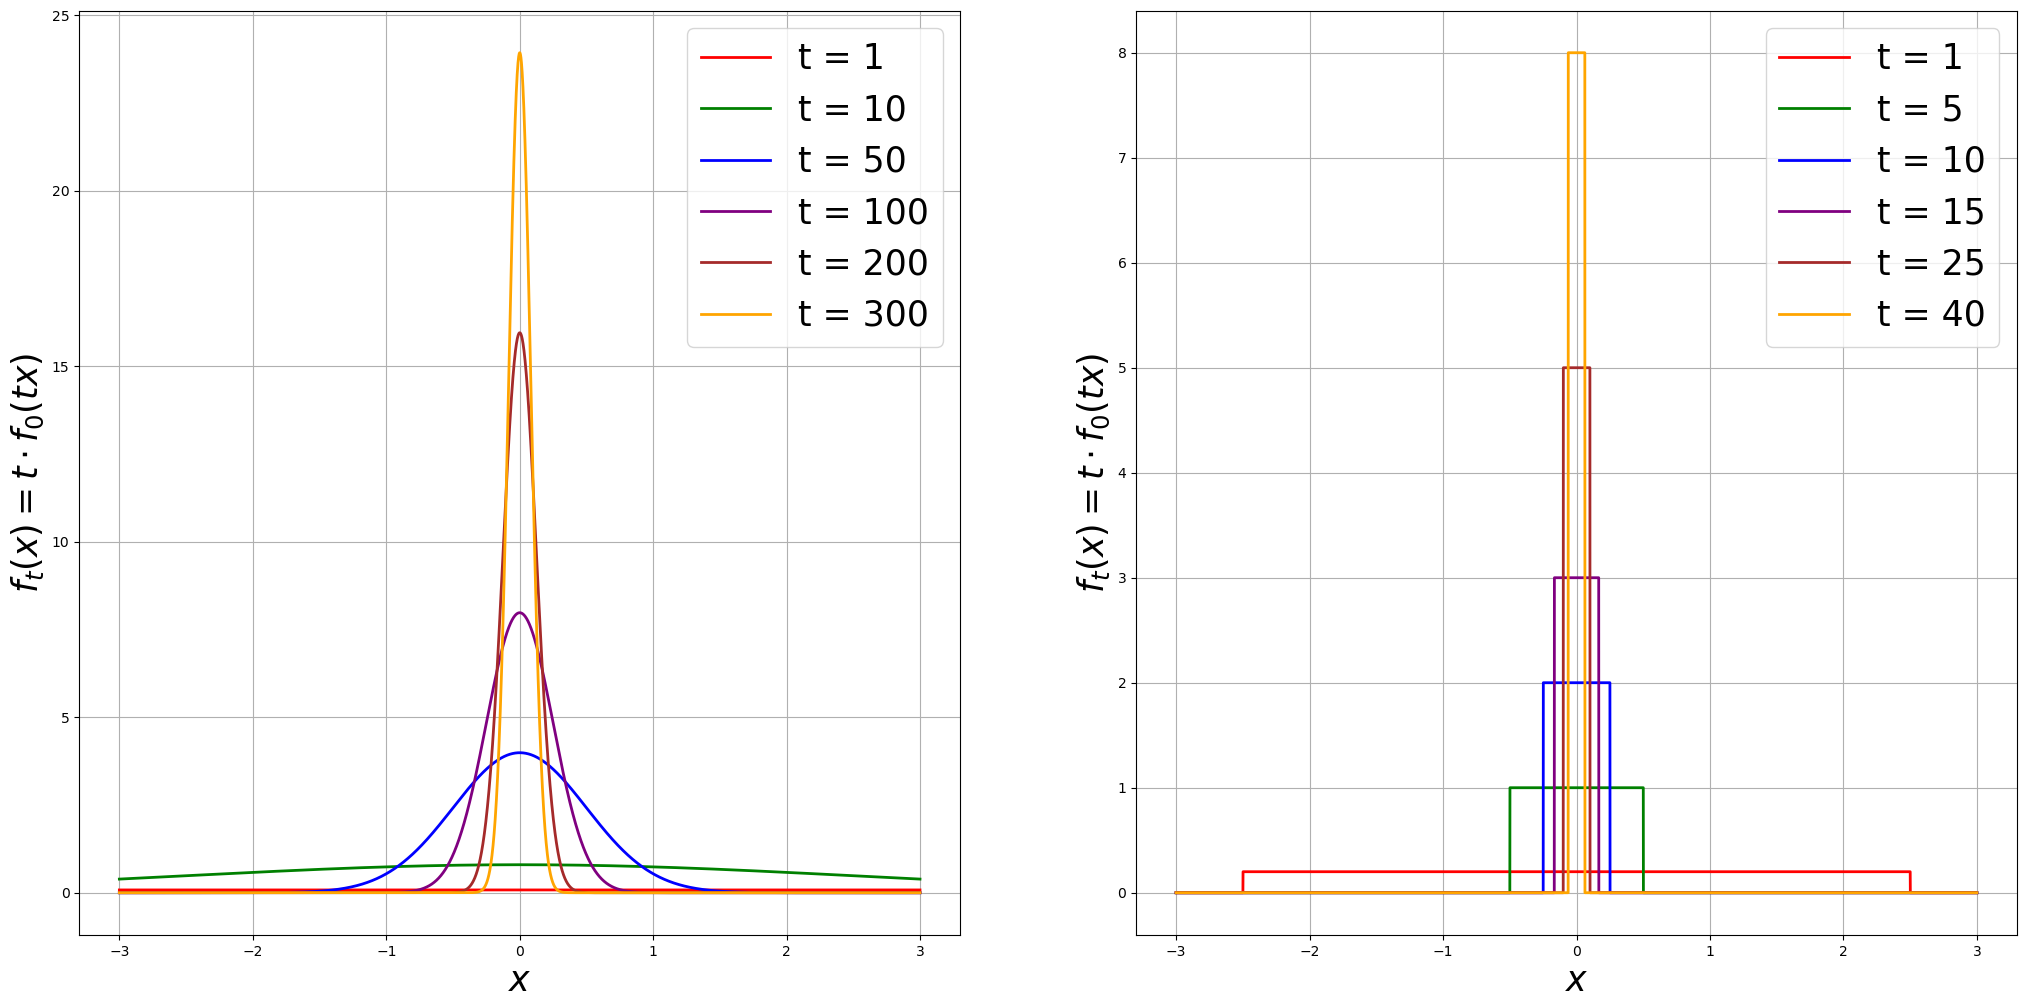
\includegraphics[width = 0.99\linewidth]{pictures/example1.png}
        \caption{Illustration of weak limit to $\delta$ function. $\mathcal{N}(0, 5)$ left, $\mathcal{U}[-2.5, 2.5]$ right.}
        \label{example1_fig}
    \end{figure}

    
    \begin{theorem}[Inequality on $\|\text{D}\|_q$] \label{ineq_q}
        Consider 
        \begin{equation}\label{f_R}
            f_A(x) = \dfrac{1}{\lambda(A)} \cdot \textbf{1}_{A}(x),
        \end{equation}

        where $A \subset \mathbb{R}^n$ is arbitrary set of a non-path measure, $\lambda(A)$ -- the measure of a set $A$.

        Then for all $A \subset \mathbb{R}^n :  0 < \lambda(A) < +\infty$ and for all $1 \leq q \leq +\infty$ such that $\text{D}(f_A) \in L_q(\mathbb{R}^n)$ is fulfilled that  

        \begin{equation}\label{int_f_R}
            \|\text{D}\|_q \geq \int\limits_{A} \text{D}(f_A)(x)dx
        \end{equation}
    \end{theorem}
    
    \begin{proof}
        First of all let's calculate $\|f_A\|_p$:

        \begin{equation*}
            \|f_A\|_p = \left( \text{ } \int\limits_{\mathbb{R}^n}\left(\dfrac{1}{\lambda(A)}\right)^p \cdot \textbf{1}_{A}(x) dx \text{ } \right)^{1/p} = \dfrac{1}{\lambda(A)} \cdot (\lambda(A))^{1/p} = (\lambda(A))^{-1 + 1/p}
        \end{equation*}

        So, $f_A \in L_p(\mathbb{R}^n)$ for all $A \subset \mathbb{R}^n : 0 < \lambda(A) < +\infty$ and $1 \leq p \leq +\infty$. 

        Now write out a Herder's inequality. For $q$ such that $\frac{1}{p} + \frac{1}{q} = 1$ is fulfilled that

        \begin{equation*}
            \|f_A\|_p \cdot \|\text{D}(f_A)\|_q \geq \|f_A \cdot \text{D}(f_A)\|_1
        \end{equation*}

        Using common inequality on operators norm $\|\text{D}(f)\|_q \leq \|\text{D}\|_q \cdot \|f\|_q ~\forall f \in L_q(\mathbb{R}^n)$ we get

        \begin{equation*}
            \|f_A\|_p \|f_A\|_q \cdot \|\text{D}\|_q \geq \|f_A \cdot \text{D}(f_R)\|_1
        \end{equation*}

        Since $\|f_A\|_p \|f_A\|_q = (\lambda(A))^{-1 + 1/p} \cdot (\lambda(A))^{-1 + 1/q} = (\lambda(A))^{-2 + 1/p + 1/q} = (\lambda(A))^{-1}$ we get:

        \begin{equation*}
            \|\text{D}\|_q \geq \lambda(A) \cdot \|f_R \cdot \text{D}(f_A)\|_1
        \end{equation*}

        Let's look at $\|f_A \cdot \text{D}(f_A)\|_1$ in more detail:

        \begin{equation*}
            \|f_A \cdot \text{D}(f_A)\|_1 = \int\limits_{\mathbb{R}^n} \text{D}(f_A)(x) \cdot \dfrac{1}{\lambda(A)} \textbf{1}_{A}(x) dx = \dfrac{1}{\lambda(A)} \int\limits_{A} \text{D}(f_A)(x)dx
        \end{equation*}

        Finally, we get the desired inequality

        \begin{equation*}
            \|\text{D}\|_q \geq \int\limits_{A} \text{D}(f_A)(x)dx
        \end{equation*}
    \end{proof}
        

    \textbf{Discussion of Theorem \ref{ineq_q}}

    To begin with, note that the result of Theorem \ref{ineq_q} does not depend in any way on whether $\text{D}$ converts $\mathbf{R}$ to $\mathbf{R}$, it is a consequence of Herder's inequality. 
    
    If you look at it from a probabilistic point of view (so now $\text{D} : \mathbf{R} \to \mathbf{R}$), then $f_A$ is a distribution density function of vectors uniformly distributed on a set $A$. So, $\int\limits_{A} \text{D}(f_A)(x)dx \leq 1$, i.e. from Theorem \ref{ineq_q} we can only get that $\|\text{D}\|_q \geq 1$. But if $\|\text{D}\|_q \geq 1$, so $\text{D}$ wouldn't be a contraction mapping in $\|\cdot\|_q$, because there always would be function $f \in \mathbf{R}$ such that $\|\text{D}(f)\|_q \geq \|f\|_q$.

    In our experiments we will measure $\hat{F}_t(\sup(A))$ and $\hat{F}_t(\inf(A))$. If $1 \in I_{\varepsilon}[\hat{F}_t(\sup(A))]$ and $0 \in I_{\varepsilon}[\hat{F}_t(\inf(A))]$, where $I_{\varepsilon}$ is confidence interval from \eqref{inter}, then we can say that operator $\text{D}$ can't be a contraction mapping.

\section{Experiments} \label{Experiments}

    \subsection{Experiment Design} \label{design}
        We consider such a formulation of the problem of repeated supervised learning: there is an original data $\textbf{X}$ and a vector of target variables $\mathbf{y}$. Initially, at round $r = 0$, we select $30\%$ of the original dataset on which our model $H(\mathbf{x}, \theta^0, 0)$ is trained with $80\%$ train size. 
        
        Then at each step $t$ we randomly select an element $(\mathbf{x^i}, y_i)$ -- the features and target variable of the $i$-th object from the original dataset, and this element does not lie in the initial dataset. Next, we get the prediction $y'_i$ of our model on the element $(\mathbf{x^i}, y_i)$: $y_i'=H(\mathbf{x^i}, \mathbf{\theta}^r, t)$ and sample $z_i \sim \mathcal{N}(y_i', s \cdot \sigma^2)$, where $s$ is an experiment parameter that indicates adherence and $\sigma$ is the model's mean squared error on held-out data. Then we remove 1 element from the active dataset and, with the probability of $p$, we add $(\mathbf{x^i}, z_i)$ to it, and with the probability $(1-p)$ we add the element $(\mathbf{x^i}, y_i)$. We carry out this procedure until we run out of elements that were not initially included in our dataset, so, we make a total of $0.7 \cdot n$ steps, where $n$ is the number of objects in $\textbf{X}$.

        After each $T$ steps round $r$ is increasing: $r = r+1$ and the machine learning model $H(x, \theta^r, t)$ is retrained with $80\%$ train size on active dataset. 

        The size of active dataset will always be $0.3 \cdot n$, because on each step we remove 1 element and add 1 element to active data. This experiment design is similar to \cite{khritankov2021hidden} were author was detecting hidden feedback loops in machine learning systems. The scheme of the experiment is shown in Figure \ref{ex_set}.

        \begin{figure}[h!]
            \centering
            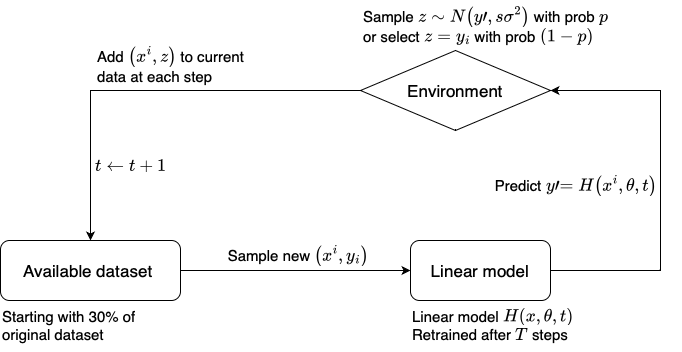
\includegraphics[scale = 0.5]{pictures/Experiment_setup.png}
            \caption{Experiment setup.}
            \label{ex_set}
        \end{figure}

        In this paper we consider linear model, that is solved as Ridge regression with mean squared error loss function. In the formulation of our experiment, we consider $\mathbf{R}$ \eqref{R} as space of density functions of random vectors $(\mathbf{x^i}, y_i)$, where $\mathbf{x^i} \in \textbf{X}$ and $y_i \in \textbf{y}$ -- the features and target variable of the $i$-th object. The operator $\text{D}$ transforms $\mathbf{R}$ at each step $t$, and the distribution of features does not change, because at each step we take new $\mathbf{x^i}_t$ from the original set of features $\textbf{X}$, so only the distribution of the target variable changes. So we can use results from Theorem \ref{delta}. 

\newpage

    \subsection{Experiment results} \label{res}

        In almost all distributions, decreasing the variance to 0 means that the distribution function takes the form of a delta function, for example in the normal distribution $\mathcal{N}(\mu, \sigma^2)$:

        \begin{equation*}
            f(x) = \dfrac{1}{\sqrt{2 \pi} \sigma} \exp\left[-\dfrac{1}{2} \cdot \left(\dfrac{x - \mu}{\sigma}\right)^2\right] \quad \text{ and } \quad \sigma^2 = \sigma^2
        \end{equation*}

        And in continuous uniform distribution $\mathcal{U}[a, b]$:
        \begin{equation*}
            f(x) = \dfrac{1}{b-a} \cdot \textbf{1}_{[a;b]} \quad \text{ and } \quad \sigma^2 = \dfrac{1}{12} \cdot (b-a)^2
        \end{equation*}

        For this reason, in our experiments every $N$ steps we measured the standard deviation in the $\mathbf{y} - \mathbf{y_{\text{pred}}}$ array, where $\mathbf{y_{\text{pred}}}$ is the predictions of our model on the active dataset. We measured the standard deviation at different \textit{usage} -- the probability with which we take $(\mathbf{x^i}, z_i)$ into the active dataset, and \textit{adherence} -- the parameter by which we multiply $\sigma^2$ when sampling $z_i$.
        
        First we consider $\mathbf{X}$ and $\mathbf{y}$ as a regression problem, so $\mathbf{y} = \mathbf{X}  \cdot \mathbf{\theta}$ for some vector $\mathbf{\theta}$. To complicate the model, a normally distributed noise was added to the data. In Figure \ref{3D} there are five 3-dimensional plots for different noise in original data, where on $X$-axis is plotted \textit{usage}, on $Y$-axis is \textit{adherence} and on $Z$ is deviation of $\mathbf{y} - \mathbf{y_{\text{pred}}}$ for test data samples.

        \begin{figure}[h!]
            \centering
            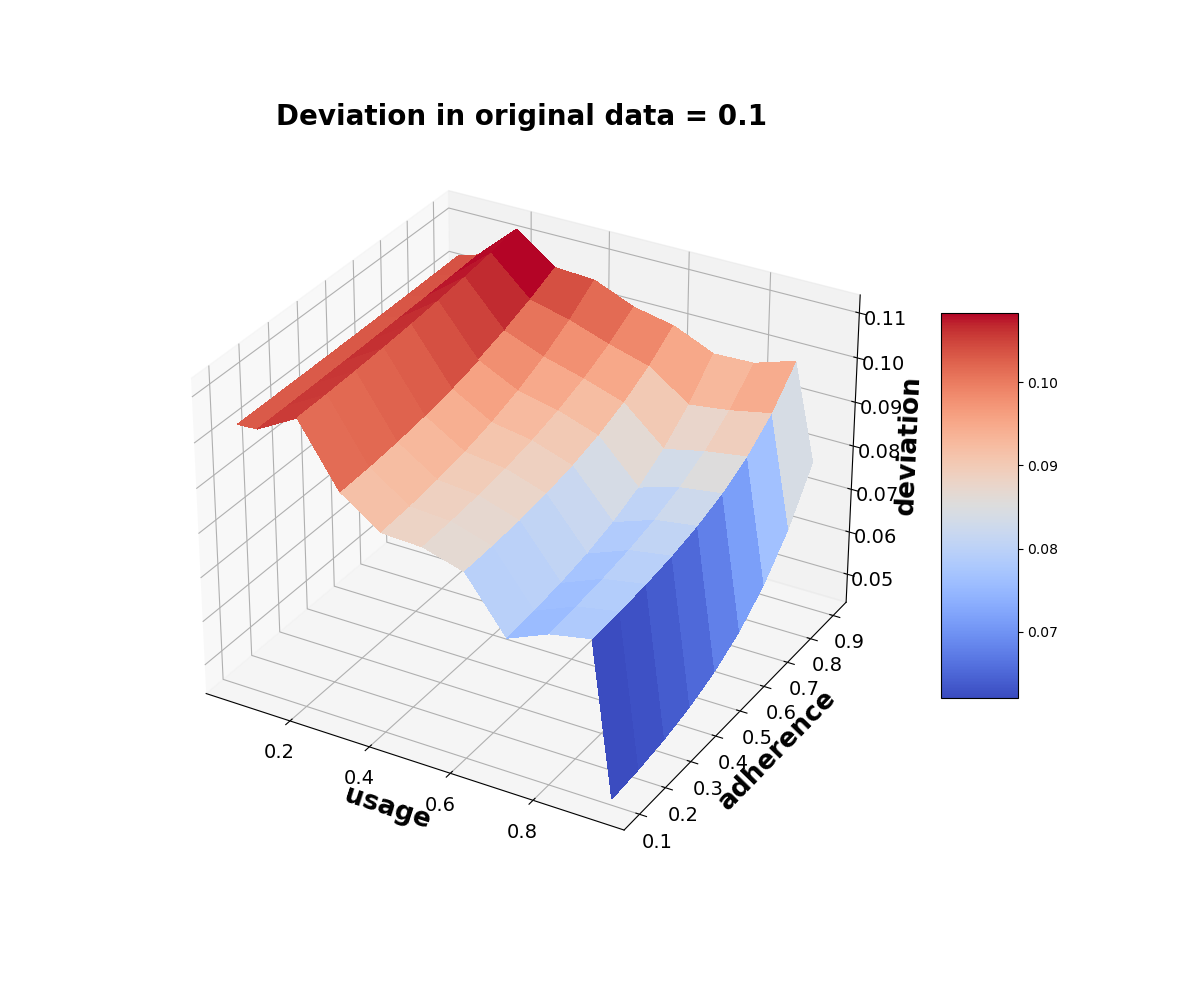
\includegraphics[width=0.33\linewidth]{pictures/3D_plot_0.1.png}
            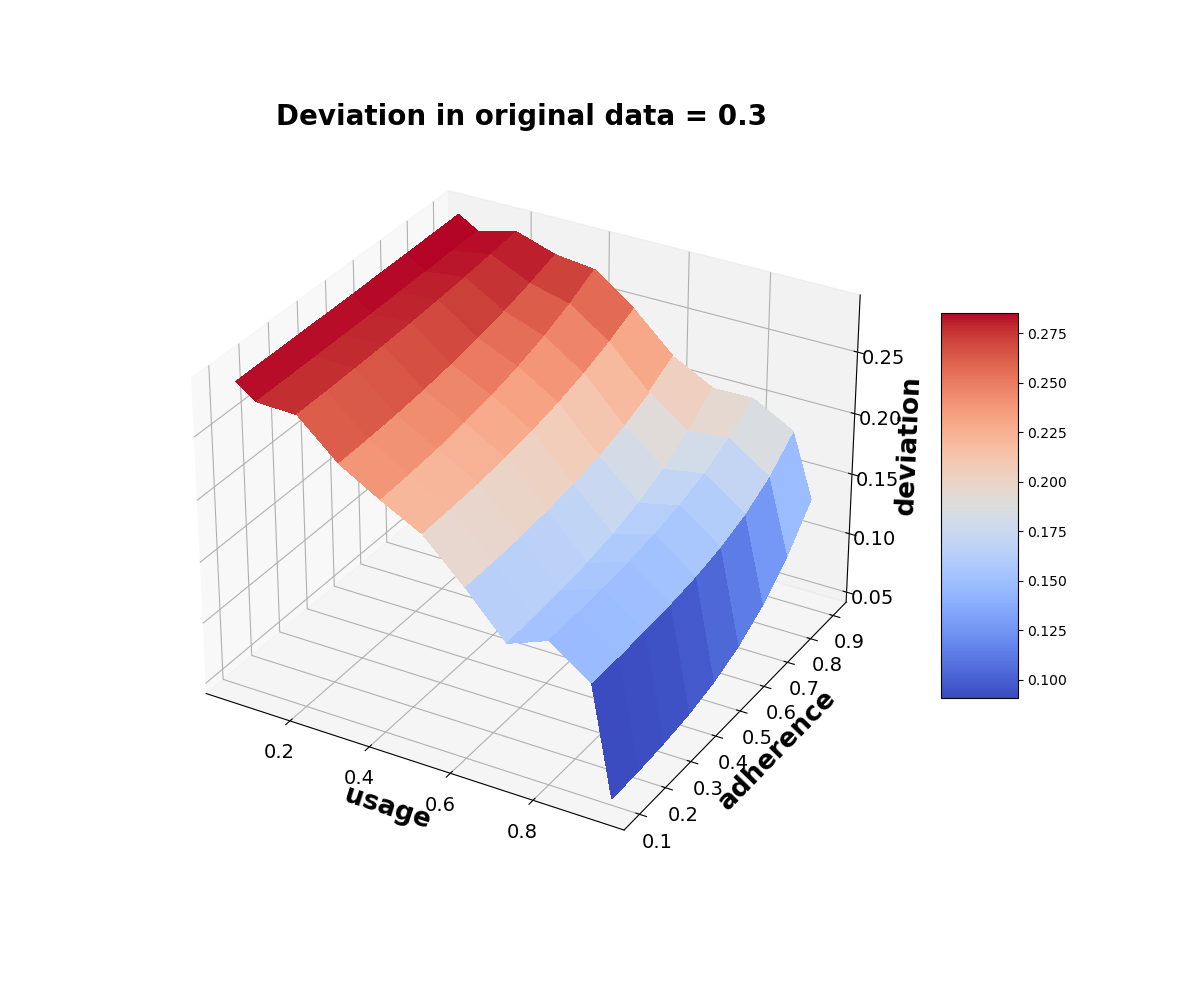
\includegraphics[width=0.33\linewidth]{pictures/3D_plot_0.3.png}
            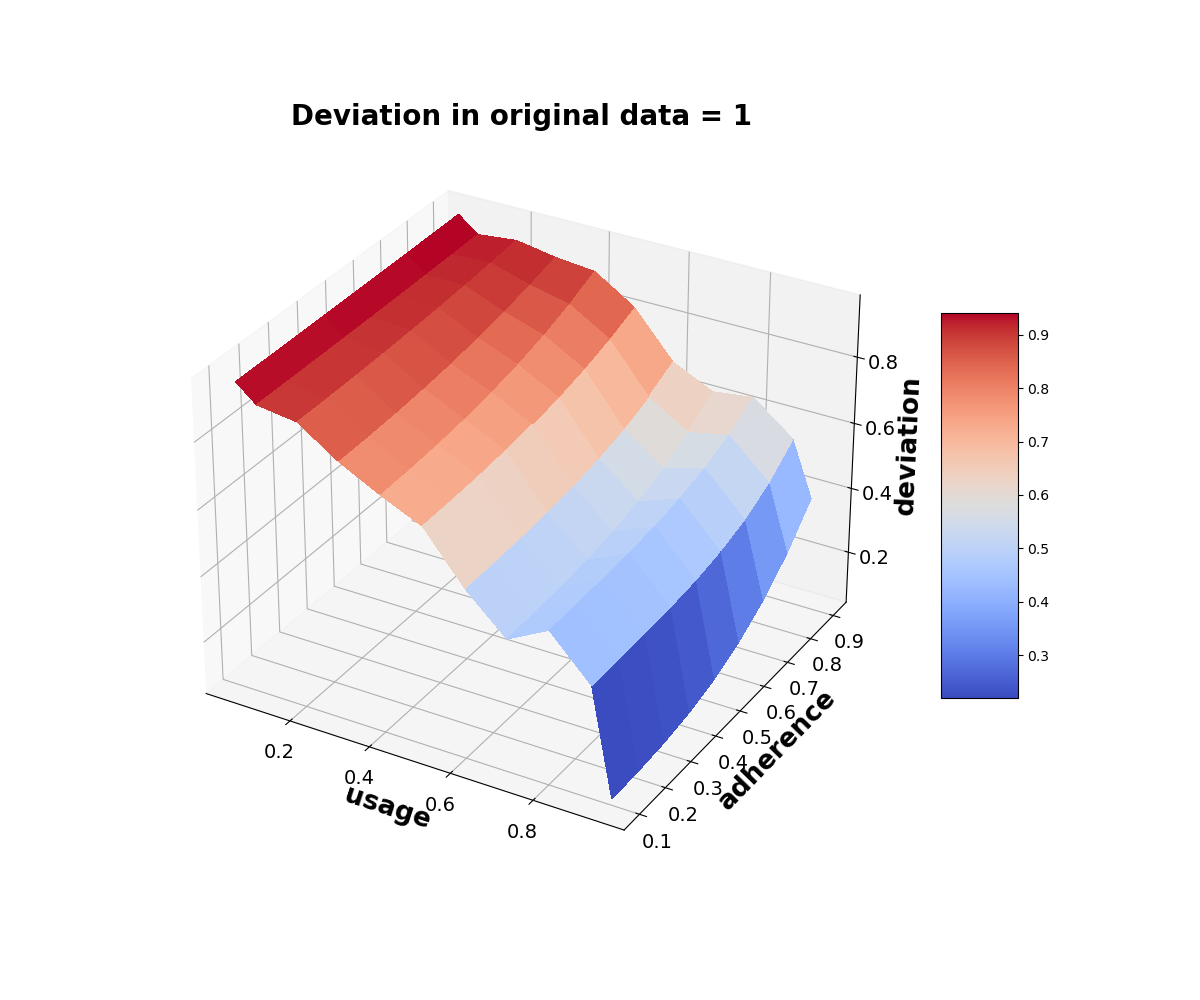
\includegraphics[width=0.33\linewidth]{pictures/3D_plot_1.png}
            
            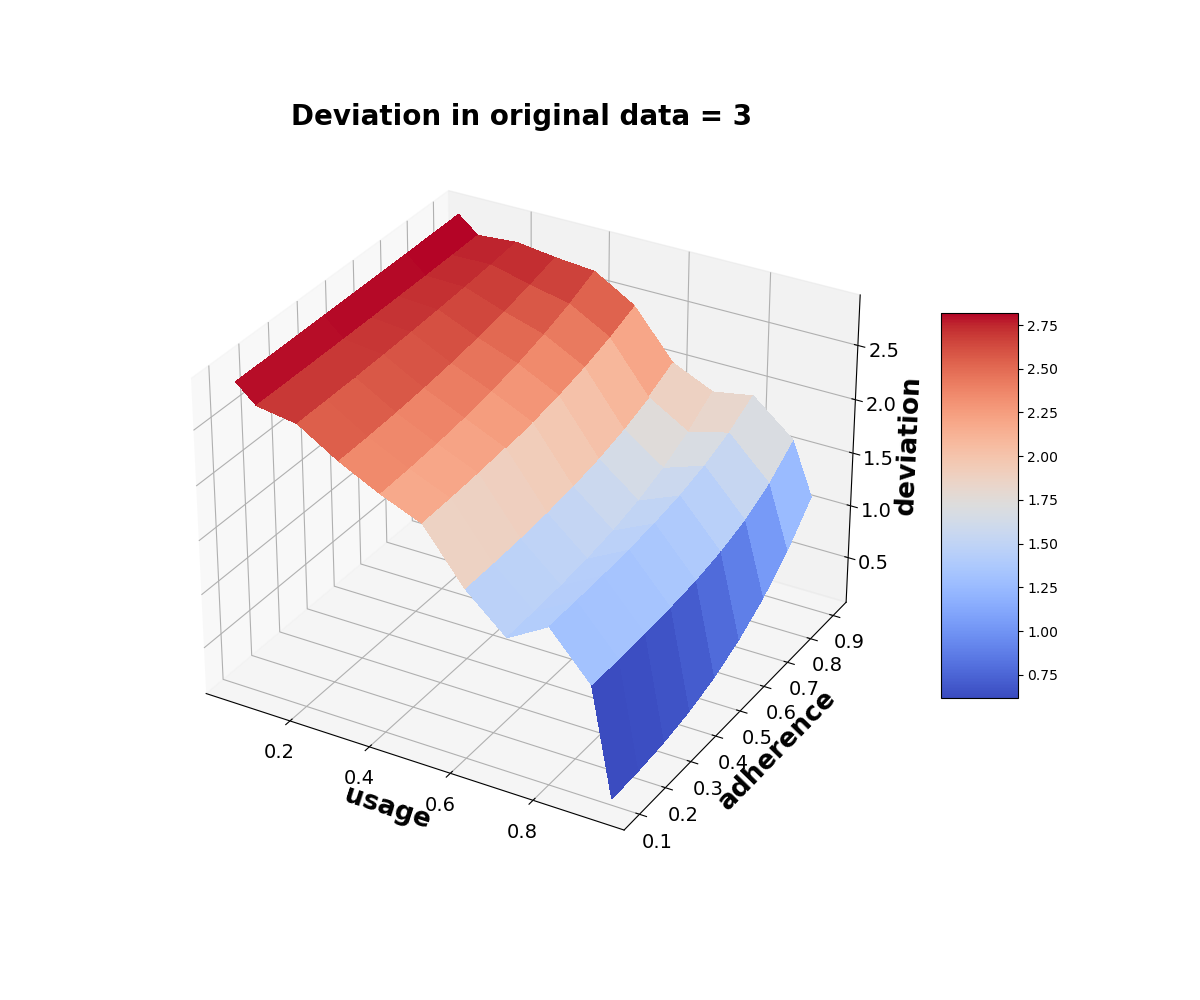
\includegraphics[width=0.33\linewidth]{pictures/3D_plot_3.png}
            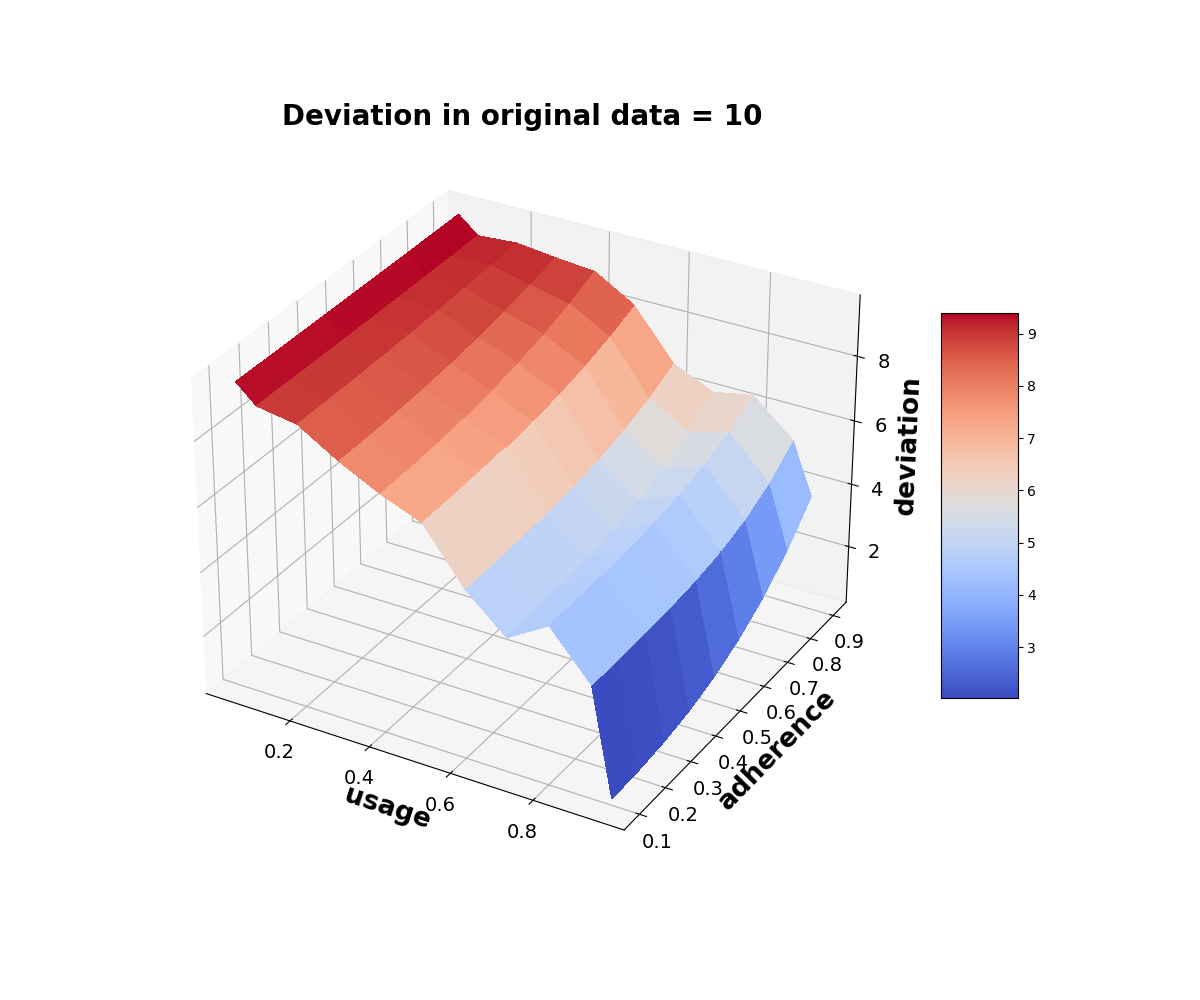
\includegraphics[width=0.33\linewidth]{pictures/3D_plot_10.png}
            
            \caption{3D Graphics for different  noise in original data}
            \label{3D}
        \end{figure}

        As we can see, the picture for the graphs at noise= $0.3, 1, 3$ and $10$ are very similar to each other, they differ only in the deviation values. This is due to the fact that for higher values of noise it becomes more profitable to add new data than to take the original data, since the noises in them are smaller, that is, with increasing \textit{usage} the deviation will fall.
        
\newpage

\bibliographystyle{plain}
\bibliography{refs}  

\end{document}